\usetikzlibrary{calc}
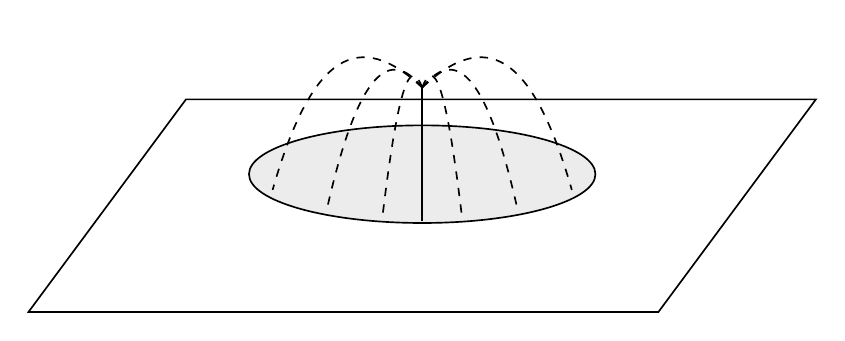
\begin{tikzpicture}[x=1cm,y=1cm,font=\normalsize,
  app edge/.style={draw=black,solid,line width=.6pt},
  app jet/.style={draw=black,dashed,line width=.6pt}]
% parallelogram lawn
\draw[app edge] (0.0000,2.7000)--(8.0000,2.7000)--(6.0000,0.0000)--(-2.0000,0.0000)--cycle;
% shaded elliptical pool
\filldraw[fill=gray!15,draw=black,line width=.6pt] (3.0000,1.7500) ellipse (2.2000 and 0.6200);
% vertical fountain pipe (base inside pool, top above back edge)
\draw[app edge] (3.0000,1.1500)--(3.0000,2.8500);
% six symmetric dashed jets from pipe top to pool interior
\draw[app jet] (3.0000,2.8500) .. controls (2.2000,3.6000) and (1.6000,3.3000) .. (1.1000,1.5500);
\draw[app jet] (3.0000,2.8500) .. controls (2.6000,3.3500) and (2.2000,3.1000) .. (1.8000,1.3500);
\draw[app jet] (3.0000,2.8500) .. controls (2.8500,3.2500) and (2.7000,2.9000) .. (2.5000,1.2500);
\draw[app jet] (3.0000,2.8500) .. controls (3.1500,3.2500) and (3.3000,2.9000) .. (3.5000,1.2500);
\draw[app jet] (3.0000,2.8500) .. controls (3.4000,3.3500) and (3.8000,3.1000) .. (4.2000,1.3500);
\draw[app jet] (3.0000,2.8500) .. controls (3.8000,3.6000) and (4.4000,3.3000) .. (4.9000,1.5500);
\end{tikzpicture}
